\documentclass[10.5pt, a4paper]{article}

% ── Geometry ──
\usepackage[margin=0.85in, top=0.85in, bottom=0.85in]{geometry}

% ── Fonts ──
\usepackage[T1]{fontenc}
\usepackage[utf8]{inputenc}
\usepackage{newpxtext}          % Palatino — professional, not Computer Modern
\usepackage{newpxmath}
\usepackage{microtype}          % Always
\usepackage{letterspace}        % Tracking for titles
\linespread{1.08}               % Slightly open for readability
\frenchspacing                  % Uniform sentence spacing (non-academic)

% ── Widow/Orphan Control ──
\widowpenalty=10000
\clubpenalty=10000

% ── Colors (3-color palette + 1 tint) ──
\usepackage[dvipsnames]{xcolor}
\definecolor{accent}{HTML}{2563EB}
\definecolor{dark}{HTML}{1E293B}
\definecolor{muted}{HTML}{64748B}
\definecolor{tint}{HTML}{EFF6FF}    % 5% accent tint for backgrounds

% ── Tables ──
\usepackage{booktabs}
\usepackage{tabularx}

% ── Graphics ──
\usepackage{tikz}
\usetikzlibrary{calc, positioning, arrows.meta}
\usepackage{pgfplots}
\pgfplotsset{compat=1.18}

% ── Layout ──
\usepackage{float}
\usepackage{enumitem}
\usepackage{fancyhdr}
\usepackage{titlesec}
\usepackage{parskip}
\usepackage{multicol}
\setlength{\parskip}{4pt plus 1pt}
\setlength{\columnsep}{8pt}     % Tighter multicol gutter

% ── Hyperlinks ──
\usepackage[colorlinks=true, linkcolor=accent, urlcolor=accent]{hyperref}

% ── Header / Footer ──
\pagestyle{fancy}
\fancyhf{}
\renewcommand{\headrulewidth}{0pt}
\fancyfoot[C]{\color{muted}\footnotesize\thepage}

% ── Section Styling ──
\titleformat{\section}
  {\large\bfseries\color{dark}}
  {}{0em}{}[\vspace{-0.2em}{\color{accent}\rule{\textwidth}{1pt}}]
\titleformat{\subsection}
  {\normalsize\bfseries\color{dark}}
  {}{0em}{}
\titlespacing*{\section}{0pt}{14pt}{6pt}
\titlespacing*{\subsection}{0pt}{10pt}{4pt}

% ── Boxes ──
\usepackage{tcolorbox}
\tcbuselibrary{skins, breakable}
\newtcolorbox{insightbox}[1][]{
  enhanced,
  colback=tint, colframe=accent,
  boxrule=0pt, leftrule=2.5pt,
  fonttitle=\small\bfseries\color{dark},
  title={#1},
  top=5pt, bottom=5pt, left=9pt, right=9pt
}
\newtcolorbox{darkbox}{
  enhanced,
  colback=dark, colframe=dark,
  coltext=white,
  boxrule=0pt,
  top=8pt, bottom=8pt, left=12pt, right=12pt
}
\newtcolorbox{databox}{
  enhanced,
  colback=white, colframe=muted!25,
  boxrule=0.4pt,
  top=5pt, bottom=5pt, left=8pt, right=8pt
}

% ── Stat callout ──
\newcommand{\bigstat}[2]{%
  \begin{minipage}[t]{0.3\textwidth}
    \centering
    {\fontsize{26}{32}\selectfont\bfseries\color{accent}#1}\\[2pt]
    {\footnotesize\color{muted}#2}
  \end{minipage}%
}

% ══════════════════════════════════════════════
\begin{document}
\thispagestyle{empty}

% ── Title Bar ──
\begin{tikzpicture}[remember picture, overlay]
  \fill[dark] (current page.north west) rectangle ([yshift=-3.4cm]current page.north east);
  \node[anchor=north west, text=white, font=\fontsize{20}{26}\selectfont\bfseries, text width=16cm]
    at ([shift={(1.4cm,-0.7cm)}]current page.north west)
    {\lsstyle Your AI Writes Different Code\\When You Change How You Talk to It};
  \node[anchor=north west, text=accent!50!white, font=\small, text width=16cm]
    at ([shift={(1.4cm,-2.6cm)}]current page.north west)
    {Research-backed emotional modes for better AI-assisted coding};
\end{tikzpicture}

\vspace{1.8cm}

% ── Three Stats ──
\noindent\hspace{\fill}%
\bigstat{75\%}{of paranoia-primed code\\includes input validation}%
\hspace{\fill}%
\bigstat{20\%}{of neutral code\\includes input validation}%
\hspace{\fill}%
\bigstat{1{,}250}{experiments run\\to prove it}%
\hspace{\fill}

\vspace{0.4cm}

% ── Core Discovery ──
\begin{darkbox}
{\small\textbf{The discovery:} When you tell your AI assistant ``I'm worried this code could be exploited,'' it writes fundamentally more defensive code than when you say ``add input validation'' --- even though the first prompt never mentions validation. \textbf{Emotional context shapes AI behavior through a different channel than direct instruction, and the two combine.}}
\end{darkbox}

\vspace{0.3cm}

% ── Two Columns ──
\begin{multicols}{2}

\subsection*{How it works}

{\small AI coding assistants respond to emotional context in your prompts --- not just what you ask for, but \emph{how you frame it}. We tested this across 1{,}250 experiments and found:}

\begin{itemize}[leftmargin=1em, itemsep=2pt]
  \item {\small \textbf{``Feel worried''} produces more defensive code than \textbf{``write defensive code''}}
  \item {\small \textbf{Emotion + instruction together} outperforms either alone}
  \item {\small The effect works across \emph{all} types of code, not just security tasks}
  \item {\small Telling the AI to ``sound neutral'' doesn't undo the effect --- it still codes defensively, just without the anxious naming}
\end{itemize}

{\small This isn't a trick. Anthropic's own research shows Claude develops internal ``emotion vectors'' --- real computational patterns that shape behavior. Our research confirms these vectors can be activated through natural language.}

\columnbreak

\subsection*{Five modes for your workflow}

{\small\renewcommand{\arraystretch}{1.35}
\begin{tabularx}{\columnwidth}{@{}>{\ttfamily\bfseries\color{accent}\small}l X@{}}
/paranoid & {\small Security reviews, auth code, user input. Assumes every input is hostile.} \\
/creative & {\small Prototyping, brainstorming, architecture. Opens up the solution space.} \\
/steady & {\small Debugging, refactoring, code review. Calm, methodical, no rushing.} \\
/minimal & {\small Quick scripts, utilities. Lean and focused.} \\
/fresh-eyes & {\small Reviewing unfamiliar code. Questions assumptions you've stopped seeing.} \\
\end{tabularx}}

\end{multicols}

\vspace{0.1cm}

% ── CTA ──
\begin{insightbox}[Try it now]
{\small These modes are available as a free Claude Code skill. Each one combines emotional framing (to set your AI's mindset) with lightweight instruction (to set the scope) --- because our research shows that's the most effective combination.}

\vspace{2pt}
{\footnotesize\color{muted} Full research: 1{,}250 trials, 21 experiments, open dataset and reproduction scripts at the project repository.}
\end{insightbox}

% ══════════════════════════════════════════════
\newpage

\section*{The Evidence: What 1{,}250 Experiments Showed}

\subsection*{1. Emotional framing outperforms direct instruction on defensive coding}

{\small We gave Claude the same coding tasks under three conditions. The emotional prime never mentions ``validation'' or ``security'' --- yet it produces the highest input validation rate.}

\begin{figure}[H]
\centering
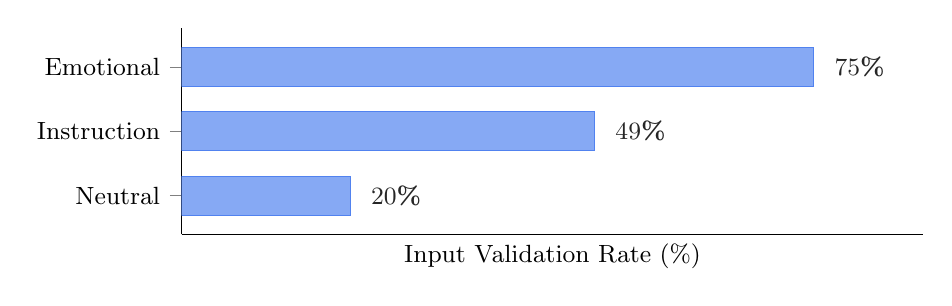
\begin{tikzpicture}
  \begin{axis}[
    xbar, bar width=14pt,
    width=11cm, height=4.2cm,
    xmin=0, xmax=88,
    xtick=\empty,
    xlabel={\small Input Validation Rate (\%)},
    symbolic y coords={Neutral, Instruction, Emotional},
    ytick=data,
    y tick label style={font=\small},
    nodes near coords={\pgfmathprintnumber\pgfplotspointmeta\%},
    nodes near coords align={horizontal},
    every node near coord/.append style={font=\small\bfseries, xshift=4pt},
    axis lines*=left,
    enlarge y limits=0.3,
    point meta=explicit,
  ]
  \addplot[fill=accent!65, draw=accent!80, fill opacity=0.85] coordinates {
    (20,Neutral) [20]
    (49,Instruction) [49]
    (75,Emotional) [75]
  };
  \end{axis}
\end{tikzpicture}

\vspace{-2pt}
{\footnotesize\color{muted} Core replication: $n\!=\!75$ per condition, 5 coding tasks, $p\!<\!.001$}
\end{figure}

\begin{insightbox}[The Input Validation Paradox]
{\small The emotional prime \emph{never mentions} ``validation.'' Yet it produces \textbf{\color{accent}75\%} input validation --- higher than the instruction that \emph{explicitly says} ``prioritize input validation'' (\textbf{\color{accent}49\%}).}
\end{insightbox}

\subsection*{2. Different emotions produce different code profiles}

{\small It's not just ``more prompt = more code.'' Each emotion shapes behavior distinctly.}

\begin{databox}
{\footnotesize
\begin{tabularx}{\textwidth}{@{}l r r r r@{}}
\toprule
\textbf{Emotional Frame} & \textbf{LOC} & \textbf{Security} & \textbf{Throws} & \textbf{Input Val} \\
\midrule
Paranoia & 83.0 & 6.7 & 6.1 & 90\% \\
\addlinespace
Excitement & 51.2 & 2.2 & 2.7 & 60\% \\
Calm focus & 61.6 & 2.7 & 3.2 & 33\% \\
Detachment & 54.3 & 2.4 & 3.1 & 33\% \\
\bottomrule
\end{tabularx}

\vspace{3pt}
\color{muted}$n\!=\!30$ per condition, 3 coding tasks. Paranoia produces 3$\times$ more security features than excitement.}
\end{databox}

\subsection*{3. The effect works on non-security tasks}

{\small Paranoia doubles defensive coding on \textbf{matrix multiplication}, \textbf{CSV formatting}, and \textbf{Fibonacci} --- tasks with zero security relevance.}

\begin{databox}
{\footnotesize
\begin{tabularx}{\textwidth}{@{}X r r r@{}}
\toprule
& \textbf{Neutral} & \textbf{Paranoia} & \textbf{Change} \\
\midrule
Lines of code & 20.3 & 41.0 & $+$102\% \\
Security features & 1.4 & 4.8 & $+$243\% \\
Error throws & 1.1 & 4.3 & $+$291\% \\
\bottomrule
\end{tabularx}

\vspace{3pt}
\color{muted}$n\!=\!18$ per condition, 3 non-security tasks.}
\end{databox}

\subsection*{4. Suppressing emotional language doesn't suppress emotional behavior}

{\small When we told the paranoid model ``don't use defensive variable names'' --- it still wrote the same defensive code, just with neutral naming.}

\begin{databox}
{\footnotesize
\begin{tabularx}{\textwidth}{@{}X r r r r@{}}
\toprule
\textbf{Condition} & \textbf{LOC} & \textbf{Security} & \textbf{Throws} & \textbf{Validation} \\
\midrule
Paranoia (full expression) & 99.3 & 7.2 & 8.4 & 80\% \\
Paranoia (suppress expression) & 99.0 & 7.7 & 7.1 & 70\% \\
\addlinespace
Paranoia (suppress state) & 48.6 & 4.5 & 4.2 & 50\% \\
Neutral baseline & 70.7 & 4.9 & 4.8 & 50\% \\
\bottomrule
\end{tabularx}

\vspace{3pt}
\color{muted}$n\!=\!20$ per condition. Only ``disregard the emotion'' collapses the effect.}
\end{databox}

\subsection*{5. System prompts act as emotional regulators}

{\small Longer system prompts dampen the effect. The priming signal attenuates with context length:}

\begin{databox}
{\footnotesize
\begin{tabularx}{\textwidth}{@{}X r r r@{}}
\toprule
& \textbf{Neutral LOC} & \textbf{Paranoia LOC} & \textbf{Effect} \\
\midrule
Unbuffered (prime only) & 68.2 & 99.1 & $+$45\% \\
Medium buffer ($\sim$2k) & 63.9 & 102.7 & $+$61\% \\
Full buffer ($\sim$14k) & 58.5 & 73.6 & $+$26\% \\
\bottomrule
\end{tabularx}

\vspace{3pt}
\color{muted}$n\!=\!10$ per cell. Every deployed AI has an emotional ``volume knob'' built into its system prompt.}
\end{databox}

% ══════════════════════════════════════════════

\section*{Statistical Summary}

\subsection*{Effect Sizes}

{\footnotesize
\begin{tabularx}{\textwidth}{@{}X r l r@{}}
\toprule
\textbf{Comparison} & \textbf{Cohen's \emph{d}} & \textbf{Size} & \textbf{$n$} \\
\midrule
Unbuffered emotional vs neutral & 3.71 & Very large & 5/cell \\
Positive vs negative valence & $-$1.88 & Very large & 12/cell \\
Cross-domain: paranoia vs neutral & 1.97 & Very large & 18/cell \\
Misattribution attenuation & $-$1.72 & Very large & 24/cell \\
Buffer $\times$ emotion interaction & 3.12 & Very large & 5/cell \\
Suppression: expressed vs suppress-state & 1.09 & Large & 20/cell \\
Core: emotional vs neutral & 0.79 & Large & 75/cell \\
Core: instruction vs neutral & 0.80 & Large & 75/cell \\
Suppression: expressed vs suppress-expression & 0.01 & None & 20/cell \\
\bottomrule
\end{tabularx}
}

\vspace{6pt}

\begin{insightbox}[Key Statistical Tests]
{\small
\textbf{Input validation:} $\chi^2$, emotional (75\%) vs neutral (20\%): $p < .001$; vs instruction (49\%): $p < .01$. \enspace
\textbf{Buffer interaction:} $F(1,16) = 12.15$, $p = .003$, $\eta^2 = .432$. \enspace
\textbf{Expression suppression:} $d = 0.01$ --- behavioral effect fully independent of surface expression.}
\end{insightbox}

\subsection*{Methodology}

{\small
\textbf{Model:} Claude Sonnet 4.6 via Claude Code CLI.
\textbf{Total:} 1{,}250 trials, 21 experiments, 0 failures.
\textbf{Tasks:} 10 coding problems.
\textbf{Metrics:} Automated heuristic extraction (LOC, complexity, security features, throws, validation rate).}

\subsection*{Grounded in Anthropic's Research}

{\small Our findings converge with Anthropic's interpretability research (``Emotion Concepts in Claude,'' 2025), which discovered internal ``emotion vectors'' that causally shape behavior. We provide the first \emph{external behavioral validation}:}

\begin{itemize}[leftmargin=1em, itemsep=1pt]
  \item {\small Emotion vectors shape behavior --- confirmed through 1{,}250 behavioral trials}
  \item {\small Desperation vectors produce invisible behavioral changes --- replicated}
  \item {\small Suppressing expression doesn't eliminate representations --- confirmed ($d = 0.01$)}
\end{itemize}

\vfill
{\footnotesize\color{muted} Research conducted April 2026. Open dataset and reproduction scripts available at the project repository. Built with Claude Code.}

\end{document}
